%----------------------------------------------------------------------------------------
%  PACKAGES AND CONFIGURATION
%----------------------------------------------------------------------------------------

\documentclass{rapport}
\usepackage{geometry}
\usepackage{fancyhdr} % For custom headers
\usepackage{lastpage} % To determine the last page for the footer
\usepackage{float}
\usepackage{extramarks} % For headers and footers
\usepackage[most]{tcolorbox} % For problem answer sections
\usepackage{graphicx} % For inserting images
\usepackage{xcolor} % For link coloring
\usepackage[hidelinks]{hyperref} % For URL links (no box or color name) 
\usepackage{amsmath}
\usepackage{algorithm}
\usepackage{algpseudocode}
%Ce que moi(Alban) ai rajouté comme package
\usepackage{comment} 
\usepackage{multicol} % Pour les colonnes
\usepackage{listings}
\usepackage{courier}
\usepackage{subcaption}

\definecolor{backcolour}{RGB}{47,47,47}
\definecolor{violet}{RGB}{200,20,200}
\definecolor{codegreen}{rgb}{0,0.6,0}
\definecolor{codegray}{rgb}{0.5,0.5,0.5}
\definecolor{marron}{RGB}{150,100,70}
\definecolor{red2}{RGB}{207,43,58}
\definecolor{bordeaux}{RGB}{74,31,30}
\lstdefinestyle{mystyle}{
    language=Python,
    basicstyle=\tiny\ttfamily
    backgroundcolor=\color{backcolour},   
    commentstyle=\color{codegreen},
    keywordstyle=\color{violet},
    numberstyle=\tiny\color{codegray},
    stringstyle=\color{red},
    literate={,}{{\textcolor{red}{,}}}1
             {;}{{\textcolor{red}{;}}}1,
    basicstyle=\ttfamily\footnotesize,
    breakatwhitespace=false,         
    breaklines=true,                 
    captionpos=b,                    
    keepspaces=true,                 
    numbers=left,                    
    numbersep=5pt,                  
    showspaces=false,                
    showstringspaces=false,
    showtabs=false,                  
    tabsize=2,
    literate=
  {á}{{\'a}}1 {é}{{\'e}}1 {í}{{\'i}}1 {ó}{{\'o}}1 {ú}{{\'u}}1
  {Á}{{\'A}}1 {É}{{\'E}}1 {Í}{{\'I}}1 {Ó}{{\'O}}1 {Ú}{{\'U}}1
  {à}{{\`a}}1 {è}{{\`e}}1 {ì}{{\`i}}1 {ò}{{\`o}}1 {ù}{{\`u}}1
  {À}{{\`A}}1 {È}{{\'E}}1 {Ì}{{\`I}}1 {Ò}{{\`O}}1 {Ù}{{\`U}}1
  {ä}{{\"a}}1 {ë}{{\"e}}1 {ï}{{\"i}}1 {ö}{{\"o}}1 {ü}{{\"u}}1
  {Ä}{{\"A}}1 {Ë}{{\"E}}1 {Ï}{{\"I}}1 {Ö}{{\"O}}1 {Ü}{{\"U}}1
  {â}{{\^a}}1 {ê}{{\^e}}1 {î}{{\^i}}1 {ô}{{\^o}}1 {û}{{\^u}}1
  {Â}{{\^A}}1 {Ê}{{\^E}}1 {Î}{{\^I}}1 {Ô}{{\^O}}1 {Û}{{\^U}}1
  {œ}{{\oe}}1 {Œ}{{\OE}}1 {æ}{{\ae}}1 {Æ}{{\AE}}1 {ß}{{\ss}}1
  {ű}{{\H{u}}}1 {Ű}{{\H{U}}}1 {ő}{{\H{o}}}1 {Ő}{{\H{O}}}1
  {ç}{{\c c}}1 {Ç}{{\c C}}1 {ø}{{\o}}1 {å}{{\r a}}1 {Å}{{\r A}}1
  {€}{{\EUR}}1 {£}{{\pounds}}1
}

\title{TS229}
\newcommand{\figsize}{1\textwidth} 

\begin{document}

%----------- Informations du rapport ---------
\logo{images/logo_em.jpg}
\unif{École nationale supérieure d'électronique, informatique, télécommunications, mathématiques et mécanique de Bordeaux}
\titre{Lecture de code-barres par lancers aléatoires de rayons}
\cours{Département Télécom} %Nom du cours
\sujet{TS225 : Projet Images} %Nom du sujet
\enseignant{Marc \textsc{DONIAS}}
\eleves{Elisa \textsc{Chien} \\
		Alban \textsc{Oberti} \\
		Tierno-Alpha \textsc{Tall} \\
		David \textsc{Yan} 
		}

%----------------------------------------------------------------------------------------
%   TITLE PAGE
%----------------------------------------------------------------------------------------
\fairemarges %Afficher les marges
\fairepagedegarde %Créer la page de garde
\newpage
\tabledematieres %Créer la table de matières
\newpage
% ------------------------------------------------ %

\section{Introduction}
Le projet présenté dans ce rapport s'intéresse à la lecture automatique des codes-barres à partir d'images. 
L'objectif principal est de développer un algorithme capable de détecter et de lire un code-barres en utilisant des techniques de traitement d'image.

D'abord, nous détaillerons les algorithmes utilisés pour la détection et la lecture du code-barres. 
Ensuite, nous expliquerons l'implémentation de ces algorithmes, puis présenterons les résultats obtenus illustrés par des exemples d'images traitées. 
Enfin, nous conclurons sur les performances globales.

\section{Algorithmes}
\begin{comment} % ref notes
~~~~ Algorithmes: ~~~~
1/
Segmentation en régions d’intérêt:
Gradients
Normalisation
Tenseur de structure local
Mesure de cohérence
Seuillage: img en niveaux de gris, on seuille
Labelisation
2/ Tierno
Extraction de l'axe:
tirage aléatoire w/ barycentre
méthode valeurs propres
 -> matrice de cov
~~~~ Implémentation: ~~~~
YCbCr
Suivi de la théorie
Optimisations (meshgrids, fonctions rapides, etc)
Optimisations: numpy et fft convolve, meshgrids
labelisation
Blob:
but: manipulation plus facile des infos
implémentation
~~~~ Résultats: ~~~~
Figures + commentaires
\end{comment}
\subsection{Détection du code barre (Phase 2)}
Dans cette première phase, nous devons détecter des zones susceptibles de contenir un code barre et tracer un rayon qui permet la lecture du code barre.

\subsubsection*{Segmentation en régions d’intérêt}
Les régions d’intérêt correspondent aux zones où il y a des codes-barres. Le code-barre présente une géométrie particulière avec de grandes bandes noires, très fines et parallèles entre elles. Cette uniformité dans la répartition des bandes et l'alternance de bandes noires et blanches se traduit par une configuration spécifique du vecteur de gradient de l’intensité de l'image.
\newline \newline L’algorithme vise à mettre en évidence cette configuration. Pour cela, nous allons calculer le tenseur de structure local. Ce tenseur nous permettra de calculer une mesure de cohérence, qui nous permettra d'évaluer si une certaine région ou structure dans l'image présente une uniformité ou une régularité dans ses caractéristiques. Elle nous permettra de détecter la géométrie particulière du code-barre.

\begin{figure}[h!]
\centering
\[
T(x, y) =
\begin{bmatrix}
T_{xx}(x, y) & T_{xy}(x, y) \\
T_{xy}(x, y) & T_{yy}(x, y)
\end{bmatrix}
\]
\caption{Tenseur de structure local}
\end{figure}
Cette matrice permet de mettre en évidence des zones de concentrations importantes de transitions entre pixels sombres et clairs; autrement dit l'alternance des barres dans un code barre.
\begin{figure}[h!]
\[
T_{ab}(x, y) = \int_{-\infty}^{\infty} \int_{-\infty}^{\infty} W(u, v) I_a(x + u, y + v) I_b(x + u, y + v) \, du \, dv
\]
où \texttt{W(x,y)} est la fonction bidimensionnelle de pondération du voisinage au point (\texttt{x}, \texttt{y}) et \texttt{I(x,y)} le vecteur gradient d'intensité.
\caption{Coefficient du tenseur de structure local}
\end{figure}


Pour calculer la mesure de cohérence, nous allons devoir d'abord calculer les vecteurs gradient d'intensité de l'image, ainsi que la fonction de pondération du voisinage pour pouvoir former le tenseur de structure local. Ensuite, la mesure de cohérence se calcule avec les coefficients du tenseur. Pour avoir de meilleur résultat, nous avons normalisé les vecteurs gradient d'intensité de l'image. Enfin, pour obtenir les régions d’intérêts, nous effectuons un seuillage sur la mesure de cohérence.
% Faut il parler de la normalisation des vecteur dans la partie implementation comme pour l'ajout de bruit pour avoir moins de regions d'interet parasite
\begin{figure}[h!]
\[
D(x, y) = \sqrt{\frac{\left(T_{xx}(x, y) - T_{yy}(x, y)\right)^2 + 4\left(T_{xy}(x, y)\right)^2}{T_{xx}(x, y) + T_{yy}(x, y)}}
\]
\caption{Mesure de cohérence}
\end{figure}
Cette dernière permet de garder seulement les régions structurées (et donc probables de contenir un code barres) de manière ordonnées parmi les zones d'intérêt candidates. 
\subsubsection*{Tracé d'un segment traversant le code barre}
Après avoir obtenu les différentes régions d’intérêt, nous les labélisons pour pouvoir effectuer les manipuler.
% quoi d'autre a rajouter
Ce processus nous permet d'obtenir un nuage de points. 
On peut dès cette étape tracer des rayons qui le traversent en son centre, de façon aléatoire ou régulière.
En outre, une méthode plus astucieuse consiste en l'extraction d'informations sur la forme de du nuage de points à partir de sa matrice de covariance. 
%Ensuite, nous récupérons le vecteur propre correspondant à la longueur du code barre, afin de tracer un segment qui traverse le code barre dans sa longueur et ainsi obtenir des couples de points pour la phase 2.
%ajouter fig
%On peut voir ce nuage comme un vecteur aléatoire de matrice de covariance
\begin{figure}[h!]
$$\Sigma = \begin{pmatrix} \text{Var}(X) & \text{Cov}(X, Y) \\ \text{Cov}(Y, X) & \text{Var}(Y) \end{pmatrix}$$
\caption{Matrice de covariance $\Sigma$}
\end{figure}
%D et u1 u2
%rôles des valeurs et vecteurs propres
%lam pour dispersion autour de u1 et u2 
En diagonalisant celle-ci, on obtient:
\begin{figure}[h!]
$$\mathbf{D} = \begin{pmatrix} \lambda_1 & 0 \\ 0 & \lambda_2 \end{pmatrix} \text{et } \quad (u_1,u_2) \quad \text{les vecteurs propres associés}$$
\caption{Diagonalisation de $\Sigma$}
\end{figure}
$\lambda_1$ caractérise la dispersion des points du nuage autour de l'axe définit par $u_1$, et $\lambda_1$ la dispersion autour de l'axe défini par $u_2$.
En effet, les valeurs propres sont homogènes à une variance, et par conséquent leurs racines carrées permettent de mesurer approximativement la largeur du nuage. En particulier, on utilise la valeur propre la plus grande $\lambda_{max}$ pour déterminer la largeur du code barre, et le vecteur propre $u_min$, associé à la valeur propre minimale $\lambda_{min}$ pour calculer son orientation
\begin{figure}[H]
    \centering
    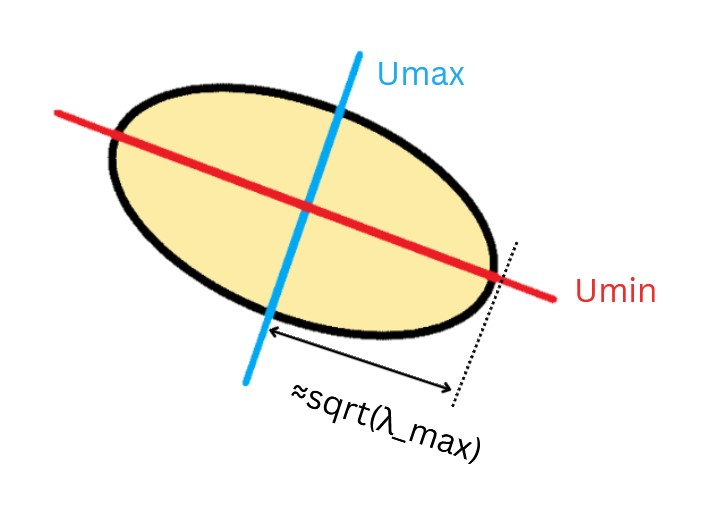
\includegraphics[width=0.5\linewidth]{images/Detection/nuage_leg.jpg}
    \caption{Schéma d'un nuage de points et des axes correspondants}
    \label{fig:nuage}
\end{figure}
C'est en utilisant ces informations qu'on est capable de tracer un rayon qui traverse le code barre dans sa largeur, en suivant le procédé ci-dessous.
\begin{algorithm}
\caption{Calcul de l'axe et du rayon}
\begin{algorithmic}[1]
\Procedure{Calcul du rayon pour un nuage donné}{}
    \State \textbf{Entrées:} $k$ \Comment{facteur d'ajustement}
    \State Calculer les valeurs propres $\lambda_1, \lambda_2$ et les vecteurs propres associés $u_1$ et $u_2$
    \State Comparer les valeurs propres pour déterminer $\lambda_{min}$ et $\lambda_{max}$
    \State Extraire le vecteur propre $u_{min}$ associé à la valeur propre minimale $\lambda_{min}$
    %\State Normaliser ce vecteur propre : $u_{min}^{(norm)}$ $ \gets \frac{u_{min}}{\|\| u_{min}\|_2}$
%    \State Calculer l'angle avec l'horizontale : $\alpha \gets \arccos(\text{axe\_norm}[0])$
    \State Calculer la longueur approximative du nuage de points : $r \gets k \cdot \sqrt{\lambda_{{\text{max}}}}$
    \State Calculer $ray \gets r \times \frac{u_{min}}{\| u_{min}\|_2}$
    \State \Return $ray$
\EndProcedure
\end{algorithmic}
\end{algorithm}



% préciser que l'extraction induit une déformation
\begin{comment}
2) Tierno
Extraction de l'axe:
tirage aléatoire w/ barycentre
méthode valeurs propres
 -> matrice de cov
\end{comment}
\newpage
\subsection{Lecture du code barre (Phase 1)}

La phase précédente a permis de récupérer un ensemble de couple de points représentant des rayons. 
Pour chaque couple de points, nous déterminons d'une part les 13 valeurs du code barre, et d'autre part, nous vérifions s'il est valide ou non.

\subsubsection*{Seuillage à l'aide d'Otsu}
La méthode d'Otsu est une technique de seuillage de Nobuyuki Otsu utilisée en traitement d'images pour la segmentation binaire. 
Elle vise à séparer les pixels d'une image en deux classes distinctes : l'avant-plan et l'arrière-plan. 
Pour ce faire, on construit l'histogramme des niveaux de gris de l'image et évalue la dispersion des pixels pour chaque seuil possible. 
Le seuil optimal est celui qui maximise la variance inter-classe, assurant ainsi une séparation claire entre les deux classes. 
En pratique, le seuil calculé se situe entre les deux pics de l'histogramme.

\subsubsection*{Détermination des limites du code-barres}
La première étape de cette phase est de réduire le segment initial, de sorte que les deux nouveaux points correspondent à la première barre noire du code barre.
Pour cela, nous devons tout d'abord opérer un seuillage de l'image grâce au seuil donné par l'algorithme d'Otsu.

Cet ensemble de points va alors être binarisé grâce au seuil. C'est à dire que les points de l'image ayant une valeur inférieure au seuil vont être associés à 0 et ceux ayant une valeur supérieure au seuil vont être associés à 1.

Les points déterminant le début et la fin du code-barres sont ensuite déterminés en prenant le premier et dernier point de valeur 0.

Finalement, un dernier échantillonnage suivi d'une binarisation sur le même seuil permet de trouver la liste binaire à analyser. Cette liste devant être compatible avec les hypotheses de données auxquelles nous allons la comparer, la binarisation ce fera dans le sens contraire de la première.
C'est à dire que les points de valeurs inférieures au seuil vont valoir 1 tandis que les autres vont valoir 0.
Le nombre de point échantillonnés est calculé en prenant $N=u*95$ avec u le plus petit multiple de 95 tel que u*95>L avec L la longueur du segment du code barre

\subsubsection*{Analyse du code barre binaire}
La prochaine étape consiste à séparer les différents blocs contenu dans la liste binaire obtenu précédemment en ne gardant que ceux représentant des nombres
Pour décoder chaque blocs, ils font être comparé avec des données de décodage en adaptant celle-ci à la taille du bloc 
Le choix se fera en prenant la plus petit norme de la différence entre le bloc et les données comparés.

\begin{table}[h!]
    \centering
    \renewcommand{\arraystretch}{1.5} % Ajuste l'espacement vertical
    \begin{tabular}{|c|c|c|c|}
        \hline
        & \textbf{Élément A} & \textbf{Élément B} & \textbf{Élément C} \\ \hline
        0 & BBBNBNN & BNBBNNN & NNNBBNB \\ \hline
        1 & BBNNBBN & BNNBBNN & NNBBNNB \\ \hline
        2 & BBNBBNN & BBNNBNN & NNBNNBB \\ \hline
        3 & BNNNNBN & BNBBBNN & NBBBNNB \\ \hline
        4 & BNBBBNN & BBNNNBN & NBNNBB \\ \hline
        5 & BNNBBBN & BNNNBBN & NBBNNNB \\ \hline
        6 & BBNBNNN & BBBNBNN & NBNBBNB \\ \hline
        7 & BNNNBNN & BBNBBBN & NBBBNNB \\ \hline
        8 & BNNBNNN & BBBBBNN & NBBNBBB \\ \hline
        9 & BBBNBNN & BBNBNNN & NNNBNBB \\ \hline
    \end{tabular}
    \caption{Tableau des éléments et des séquences associées}
    \label{tab:elements}
\end{table}

Le résultat de cette analyse se traduit par une liste de 12 chiffres et d'une liste de 6 lettres (A ou B) déterminésde
de la même façon que pour les chiffres avec le tableau précédent. Cette dernière permet de déterminer le premier chiffre du code-barres

\subsubsection*{Détermination du premier chiffre du code barre}

À partir de la séquence AB obtenue, nous pouvons déterminer le premier chiffre. 
Il suffit ainsi de lire le tableau de correspondance suivant :

\begin{table}[h!]
    \centering
    \renewcommand{\arraystretch}{1.5} % Ajuste l'espacement vertical
    \begin{tabular}{|c|c|c|c|}
        \hline
        \textbf{Séquence} & \textbf{1\textsuperscript{er} Chiffre} & \textbf{Séquence} & \textbf{1\textsuperscript{er} Chiffre} \\ \hline
        AAAAAA & 0 & ABBAAB & 5 \\ \hline
        AABABB & 1 & ABBBAA & 6 \\ \hline
        AABBAB & 2 & ABABAB & 7 \\ \hline
        AABBBA & 3 & ABABBA & 8 \\ \hline
        ABAABB & 4 & ABBABA & 9 \\ \hline
    \end{tabular}
    \caption{Tableau des familles d’appartenance de la séquence}
    \label{tab:sequence}
\end{table}

\subsubsection*{Vérification de la clef de contrôle}
Pour déterminer la clé de contrôle, il faut additionner les chiffres en positions paires à trois fois la somme des
chiffres en positions impaires jusqu'au $12^{eme}$ chiffre. 
La clé est alors valable si le chiffre des unités est égal au complément à 10 du $13^{eme}$ chiffre du code.

\section{Implémentation}

\subsection{Phase 1 : Détection du code barre}
\subsubsection*{Image}
À partir d'une image en couleur RGB, nous la convertissons en YCbCr et ne gardons que le canal de luminance. En effet, un code-barre est une alternance de bandes noires et blanches, donc seul ce contraste d'intensité nous intéresse.
\newline On ajoute d'ailleurs un bruit blanc gaussien centré de variance $\sigma_{bruit}^2$ dès le chargement de l'image. Cela améliore la capacité de détection.

\subsubsection*{Mesure de cohérence}
\label{sec:coherence}
Pour le calcul de la mesure de cohérence, nous devons tout d'abord calculer les vecteurs gradients d'intensité. Pour cela, nous les calculons au moyen des filtres de Canny, ce qui correspond à appliquer un filtre convolutif gaussien avec un écart type $\sigma_g$. Cet écart type doit être relativement faible pour trouver les vecteurs de transition correspondant aux barres blanches et noires.

Ensuite, nous calculons la fonction de pondération du voisinage à l'aide d'un filtre passe-bas gaussien, avec un écart type $\sigma_t$. Cet écart type doit être proportionnel à la taille du code-barre par rapport à la taille de l'image pour trouver des clusters de vecteurs gradient d'intensité.

\subsubsection*{Labélisation}
La labélisation des objets détectés dans l'image binaire est réalisée à l'aide de la fonction \texttt{measure.label} de la bibliothèque \texttt{skimage}. Cette fonction attribue un label unique à chaque blob extrait par le biais des étapes précédentes, permettant ainsi de les distinguer et de les analyser individuellement. À l'aide de celle-ci, nous obtenons une image labélisée accompagnée du nombre total d'objets détectés. Finalement, on obtient le nuage de points correspondant à toutes les régions potentiellement intéressantes qui ont été détectées.

De plus, pour éviter d'avoir des zones d'intérêt parasites, on rajoute sur l'image d'origine, avant le traitement d'image, un bruit blanc gaussien pour réduire la qualité de l'image. En effet, ce bruit va perturber les zones de faux positifs sans trop perturber le code-barre puisque sa structure est très contrastée.

\subsubsection*{Classe Blob}
Une fois les différentes régions extraites de l'image, il nous fallait être en capacité de tracer des rayons pour la lecture. C'est dans cet esprit que nous avons implémenté une classe \textit{Blob}. Celle-ci fournit une interface qui permet à l'utilisateur d'obtenir toutes les données utiles relatives à un blob sans qu'il ait à se soucier de l'implémentation. Ceci nous permet de produire un code plus synthétique et de fluidifier l'échange entre les deux équipes de projet.
\newline \newline Une instance de \textit{Blob} contient une batterie d'attributs nécessaires au calcul des éléments essentiels pour le tracé : on peut citer le barycentre, la matrice de covariance, ses valeurs et vecteurs propres, etc. Ces attributs sont accompagnés de méthodes qui implémentent plusieurs approches pour le tracé d'un rayon sur un blob donné. On peut par exemple tracer des rayons aléatoires qui passent par le barycentre du blob, ou un rayon de taille adéquate aligné sur l'axe du code-barre tout en étant capable d'ajuster sa longueur pour tenir compte de la déformation induite par le processus d'extraction des zones d'intérêt.
\newline \newline On peut aussi, à travers cette interface, aisément ajouter des méthodes de calcul qui permettraient d'affiner la détection : par exemple, pour utiliser d'autres approches pour le calcul du rayon, ou l'ajout de filtres sur la forme du blob pour quantifier une probabilité qu'il soit ou non un code-barre. Elle présente aussi l'avantage d'être simple d'utilisation : l'utilisateur fournit la taille d'une image et un nuage de points en son sein en entrée, et peut ensuite directement obtenir les données qui lui sont utiles.

\subsubsection*{Complexité temporelle}
Nous nous sommes efforcés de produire un code relativement efficace en termes de complexité temporelle.\newline
Initialement, celui-ci se terminait en une trentaine de secondes. 
Nous avons utilisé, dès que possible, des calculs matriciels plutôt que des boucles imbriquées, et fait un usage extensif des fonctionnalités de \textit{numpy}, qui fournit des fonctions efficaces pour les calculs d'algèbre linéaire. Le changement le plus impactant a été l'ajout de la fonction \textit{fftconvolve} de \textit{scipy}, qui tire parti de l'algorithme de la Transformée de Fourier Rapide pour effectuer des convolutions en un temps record.
\newline Ces améliorations nous ont permis d'atteindre une exécution de l'ordre d'une seconde.

\begin{comment}
Une fois les différentes régions extraites de l'image, nous développons une interface qui permet d'obtenir facilement des tracés de rayons. Nous devons être en capacité de tracer des rayons pour la lecture. C'est dans cet esprit que nous implémentons une classe \textit{Blob}. Celle-ci fournit une interface qui permet à l'utilisateur d'obtenir toutes les données utiles relatives à un Blob sans qu'il ait à se soucier de l'implémentation. Cela nous permet de produire un code plus synthétique et de fluidifier l'échange entre les deux équipes.

Une instance de \textit{Blob} contient une batterie d'attributs nécessaires au calcul des éléments essentiels pour le tracé : le barycentre et la diagonalisation de la matrice de covariance.
\end{comment}
\subsection{Phase 2 : Lecture du code barre}

Contrairement à la phase précédente, nous avons implémenté la phase 2 entièrement en programmation impérative.
Chaque étape clé de l'algorithme est implémentée par une fonction spécifique, tout en respectant les principes de modularité et de réutilisabilité du code.

\vspace{0.5cm}

Les fonctions réutilisées sont : 
\begin{itemize}
	\item \texttt{distance} : Calcule la distance entre deux points.
	\item \texttt{echantillonnage} : Échantillonne un segment pour un nombre de points donné en choisissant le plus proche voisins avec np.around.
	\item \texttt{norme\_binaire} : Calcule la norme binaire entre les blocs binaires du code-barres et les séquences à comparer. Cette norme se traduit dans l'implémentation par une comparaison bit à bit.
\end{itemize}

\vspace{0.5cm}

Les fonctions implémentées sont :
\begin{itemize}
	\item \textbf{Seuillage à l'aide d'Otsu} : La fonction \texttt{otsu} permet de seuiller une image en niveaux de gris en utilisant la méthode d'Otsu.
	D'abord, l'algorithme crée un histogramme de l'image. Ensuite, il parcourt tous les seuils possibles (de 0 à 255 dans notre cas), puis met à jour les valeurs des probabilités de classe et des moyennes de classe. 
	Dès lors, il calcule la variance inter-classe et vérifie itérativement s'il est maximal. En effet, minimiser la variance intra-classe revient à maximiser la variance inter-classe.
	\item \textbf{Détermination des limites du code-barres} : La fonction \texttt{find\_lim} permet de déterminer les limites du code barre à partir d'un segment donné. 
	La fonction \texttt{find\_u} permet de déterminer le facteur u pour échantillonner le second segment de code barre.
	\item \textbf{Analyse du code barre binaire} : La fonction \texttt{separate} détermine les douze blocs de données (ignorant les gardes) à partir du segment seuillé et les placent dans un tableau, facilitant alors le déchiffrement. 
	La fonction \texttt{compare} va alors utiliser la fonction \texttt{norme\_binaire} pour comparer chaque bloc binaire du tableau sortant de \texttt{separate} et permettre de récupérer les 12 chiffres décodés et une liste contenant la séquence AB.
	\item \textbf{Détermination du premier chiffre du code barre} : La fonction \texttt{first\_one} permet de déterminer le premier chiffre du code barre à partir de la séquence AB.
	\item \textbf{Vérification de la clef de contrôle} : La fonction \texttt{clef\_controle} permet de vérifier la validité du code barre en calculant la clé de contrôle.
	Elle est calculée par le produit scalaire avec le vecteur [1, 3, 1, 3, 1, 3, 1, 3, 1, 3, 1, 3]. De plus, nous avons utilisé un modulo 10 sur le complément à 10 pour prendre en compte que le complément à 10 de 0 est 0.

\end{itemize}

\section{Résultats}

\subsection{Phase 1 : Détection du code barre}

\begin{figure}[H] 
	\centering
	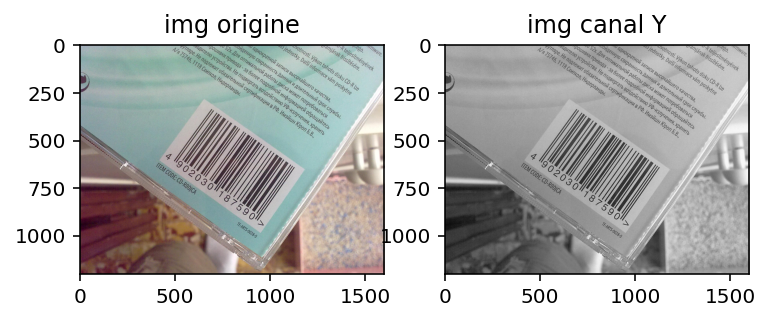
\includegraphics[width=\figsize]{images/Detection/Y.png}
	\caption{Image originale et canal de Luminance}
	\label{Y}
\end{figure}
Nous convertissons l'image couleur RGB en image canal Y pour ne garder que l'intensité du contraste. Cela nous permet de bien distinguer les bandes noires et blanches.
\begin{figure}[H] 
	\centering
	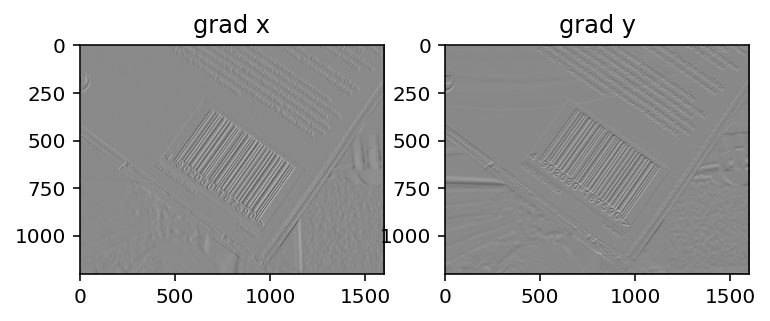
\includegraphics[width=\figsize]{images/Detection/gradients.png}
	\caption{Gradients en X et en Y}
	\label{grad}
\end{figure}
A partir du canal de luminance, nous calculons le vecteur gradient selon x et selon y. Pour vérifier qu'il s'agit du gradient selon, nous observons dans l'image à gauche, que l'on observe bien la variation horizontale d'intensité à la coordonnée (1200,1000), on donc bien un gradient selon x. Et pour l'image de droite, nous observons une variation verticale au coordonnée (0,750), donc on a un gradient selon y.
\begin{figure}[H] 
	\centering
	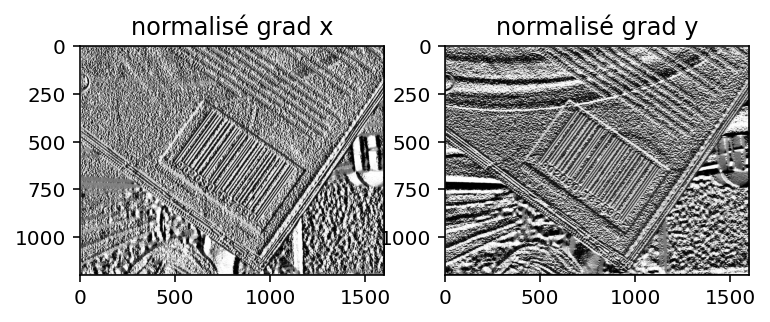
\includegraphics[width=\figsize]{images/Detection/normalisation.png}
	\caption{Normalisation des gradients}
	\label{norm}
\end{figure}
La normalisation permet d'appuyer les transitions de pixel pour faciliter la détection des codes barres et permet d'avoir un tenseur de structure local bien contrasté. 
\begin{figure}[H] 
	\centering
	\includegraphics[width=\figsize]{images/Detection/tenseur.png}
	\caption{Visualisation des composantes du tenseur de structure local}
	\label{tenseur}
\end{figure}
En observant le tenseur Txy, on peut observer la zone du code barre très contrasté par rapport au reste de l'image.

\begin{figure}[H]  
	\centering
	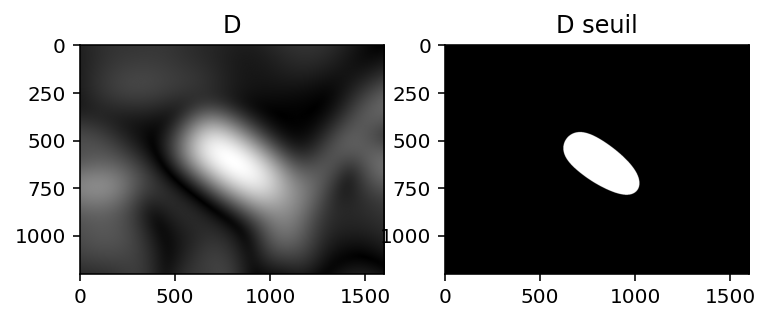
\includegraphics[width=\figsize]{images/Detection/mesure_coherence_seuil.png}
	\caption{Mesure de cohérence et seuillage }
	\label{seuil}
\end{figure}
La mesure de cohérence seuillée met en évidence une région d'interet, qui correspond à la zone où le code barre se situe. Nous effectuons un seuillage pour mettre en évidence la zone d'interêt et ainsi faciliter la labélisation.
\begin{figure}[H]  
	\centering
	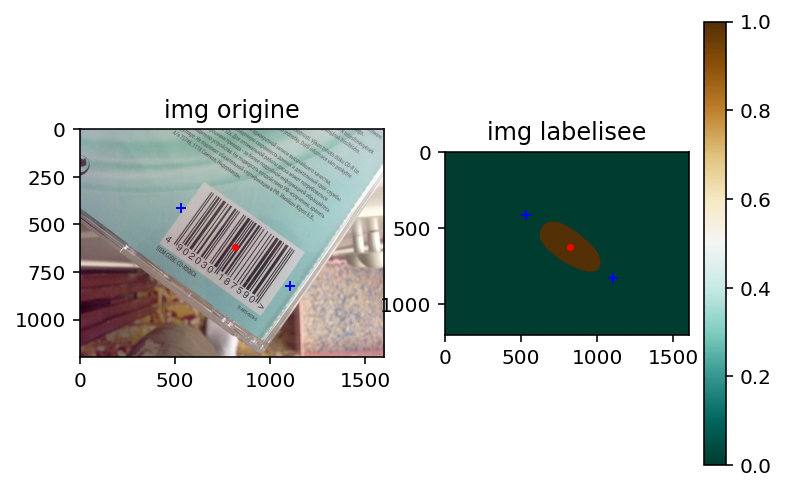
\includegraphics[width=\figsize]{images/Detection/img_labeled.png}
	\caption{Labélisation et tracé de rayon}
	\label{seuil}
\end{figure}
En choisissant des paramètres adéquats:
%$\sigma_g=2$,$\sigma_t=50$,$seuil=0.7$, $sigma_{bruit}=2$
$$\sigma_g = 2, \quad \sigma_t = 50, \quad \text{seuil} = 0.7, \quad \sigma_{\text{bruit}} = 2$$
On est obtient un tracé de rayon pertinent.
\newline Ces paramètres sont différents pour chaque image et doivent respecter les conditions citées en \ref{sec:coherence}
\begin{figure}[H]  
	\centering
	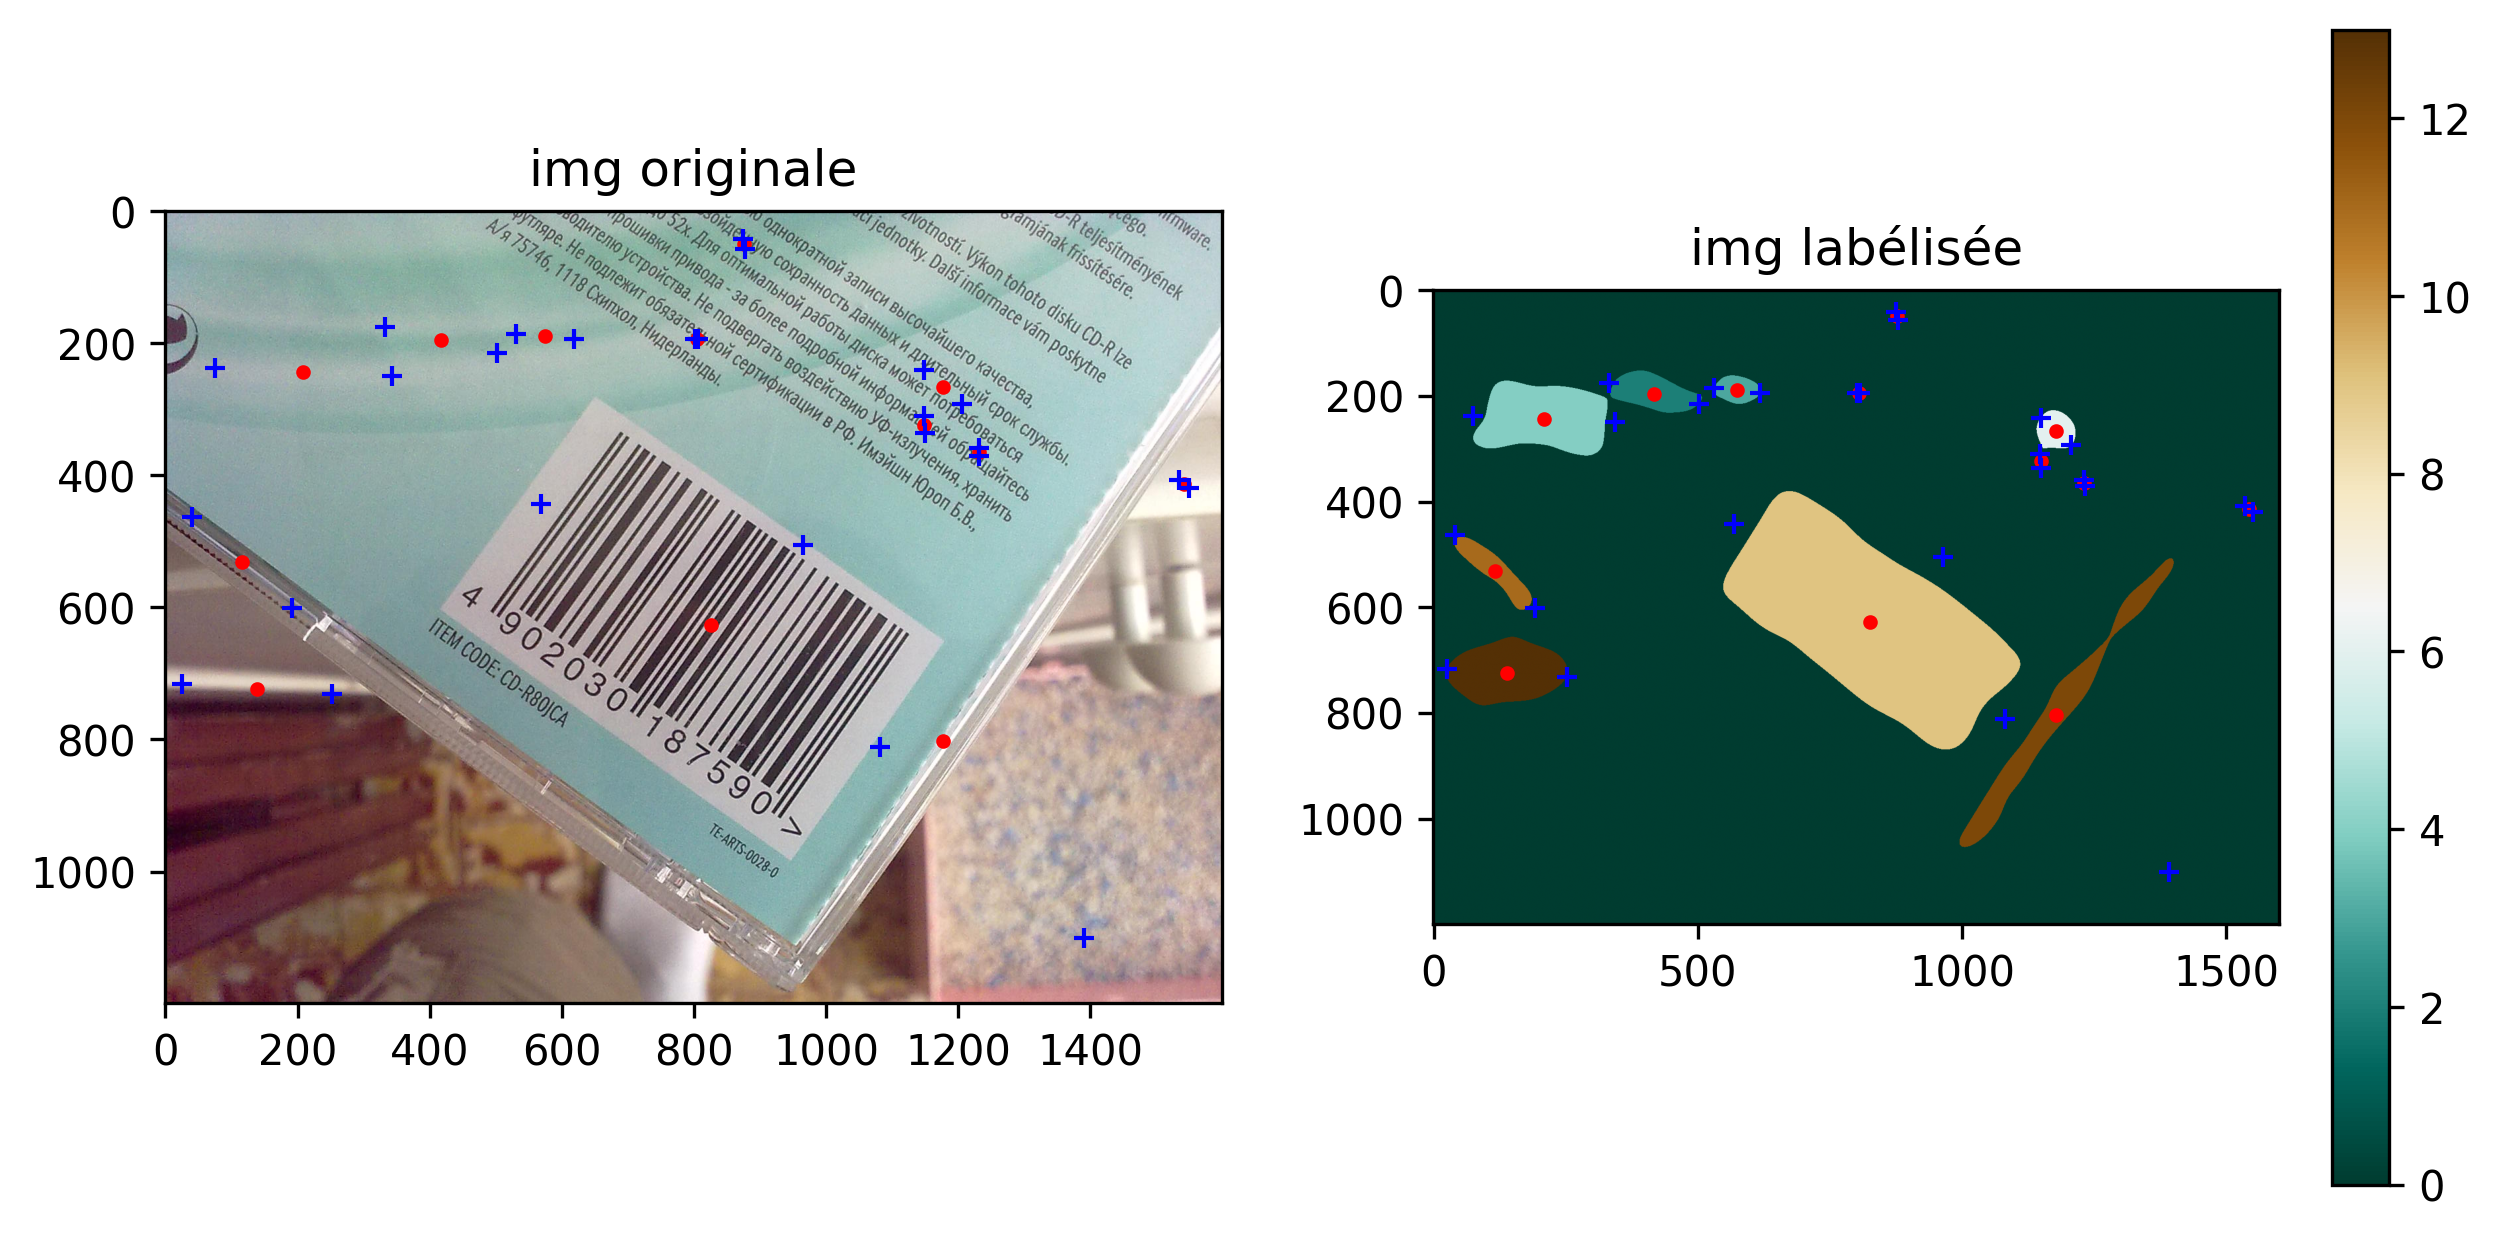
\includegraphics[width=\figsize]{images/Detection/manyblobs.png}
	\caption{Labélisation et tracé de rayon}
	\label{seuil}
\end{figure}
Si les paramètres de détection ne sont pas bien choisis, des régions parasites font surface. Ici:
%$\sigma_g=2$,$\sigma_t=50$,$seuil=0.7$, $sigma_{bruit}=2$
$$\sigma_g = 5, \quad \sigma_t = 30, \quad \text{seuil} = 0.7, \quad \sigma_{\text{bruit}} = 2$$


\subsection{Phase 2 : Lecture du code barre}

\subsubsection*{Seuillage à l'aide d'Otsu}
Prenons l'image suivante :
\begin{figure}[H] % Ajouter les deux points reçu en argument 
	\centering
	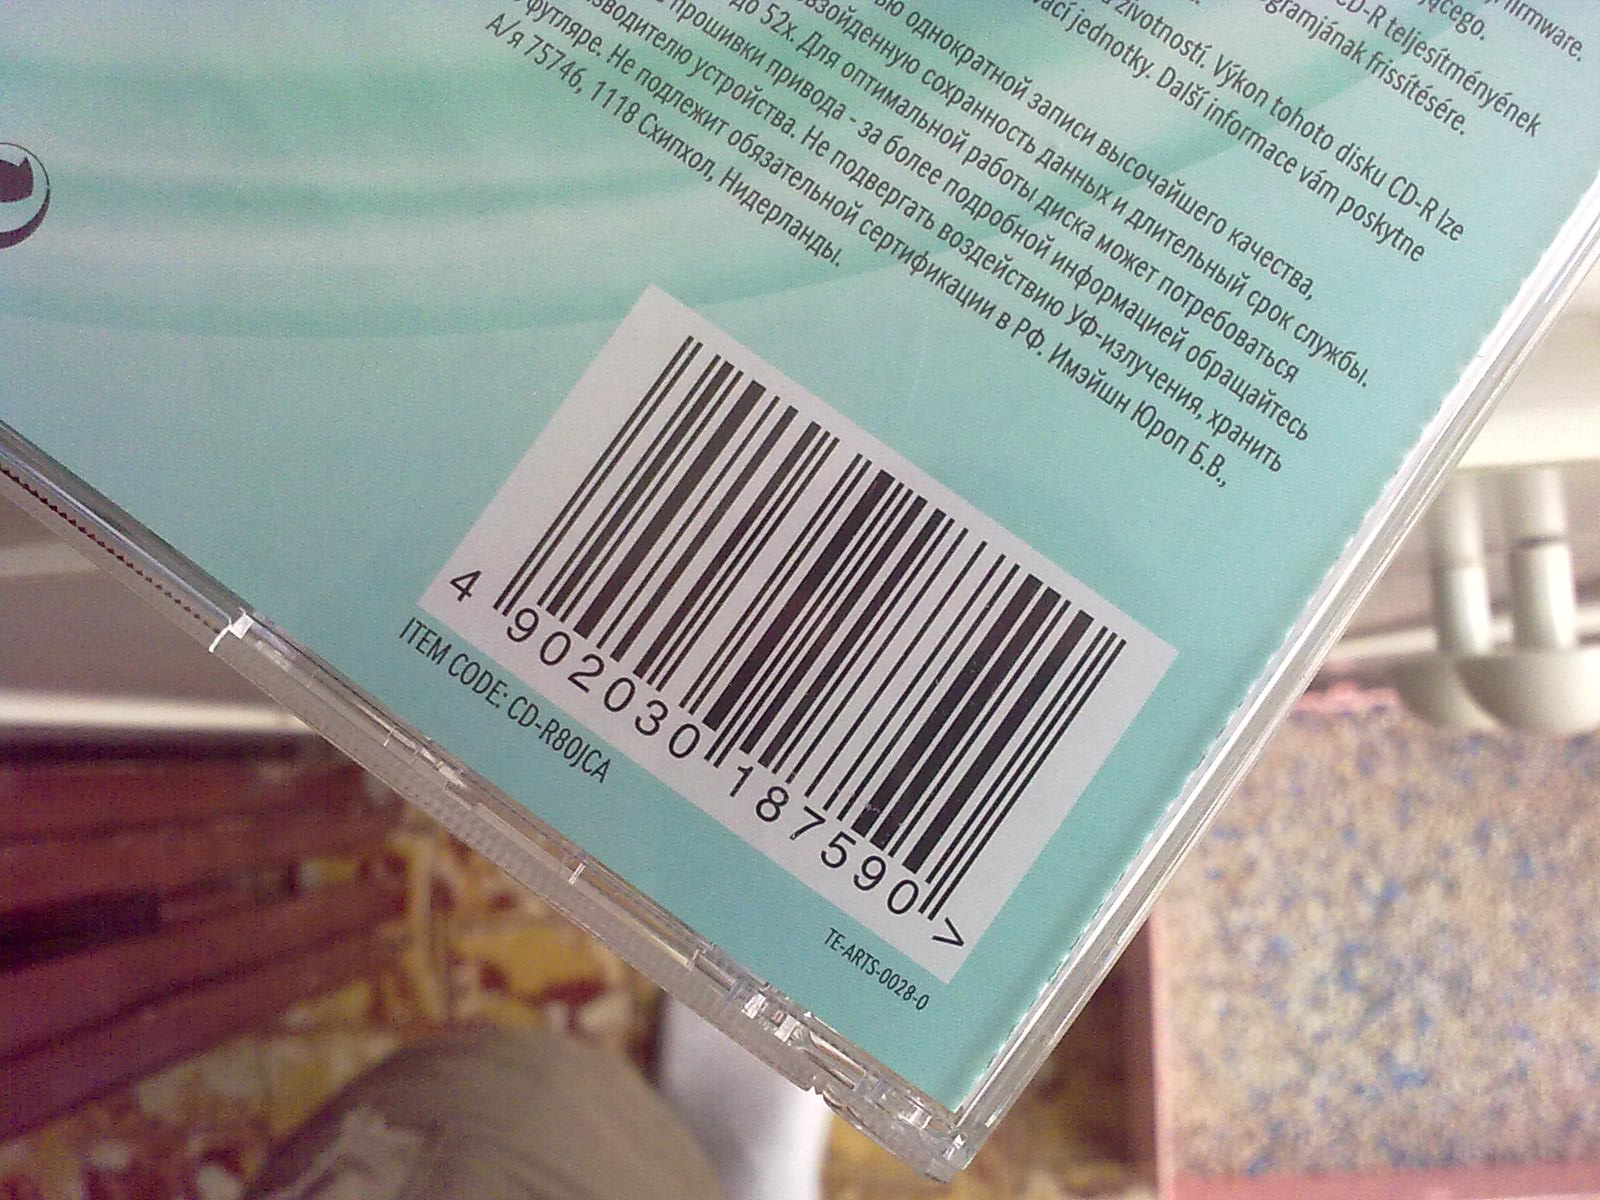
\includegraphics[width=0.5\textwidth]{images/barcode0.jpg}
	\caption{Image d'un code barre}
	\label{code_barre}
\end{figure}

Avant de pouvoir lire un code barre, nous devons opérer un seuillage de l'image. Pour cela, nous utilisons la méthode d'Otsu.
Pour rappel, cette méthode repose sur le calcul d'un seuil optimal pour binariser une image en niveaux de gris.
Ce seuil est déterminé grâce à l'histogramme de l'image et sépare les pixels en deux classes distinctes : les pixels noirs et les pixels blancs.

Pour l'image en figure \ref{code_barre}, nous obtenons l'histogramme suivant :

\begin{figure}[H] 
	\centering
	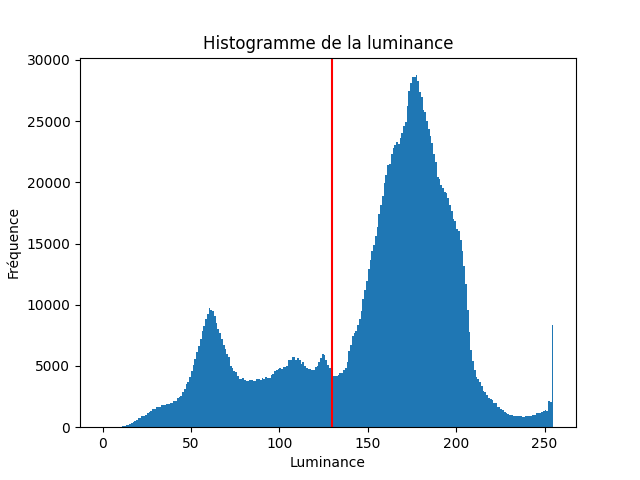
\includegraphics[width=0.5\textwidth]{images/histogramme.png}
	\caption{Histogramme de la luminance de l'image}
	\label{histogramme}
\end{figure}

Grâce à ce seuil dénoté par la barre rouge, nous obtenons ainsi l'image seuillée : 
\begin{figure}[H] 
	\centering
	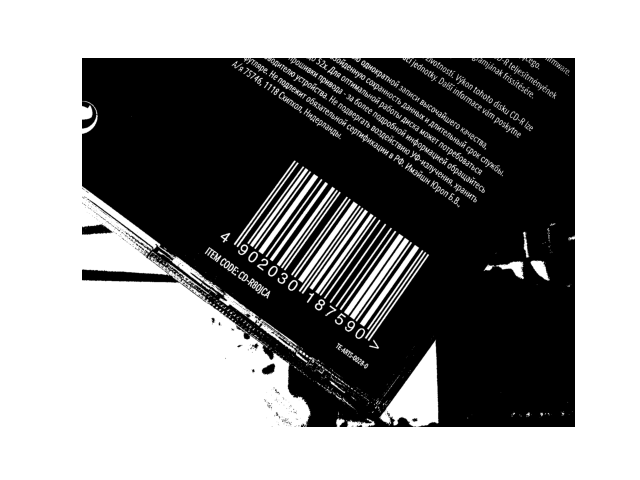
\includegraphics[width=0.5\textwidth]{images/barcode_seuillee.png}
	\caption{Image seuillée}
	\label{img_seuillee}
\end{figure}

\subsubsection*{Détermination des limites du code-barres}
Une fois le seuil déterminé, nous pouvons déterminer les limites du code barre.
La première étape consiste à un échantillonnage sur un segment puis une binarisation selon un seuil. Ce segment est visble en vert sur la figure suivante.

Nous recevons en argument deux points, qui définissent un segment sur l'image seuillée, comme représenté sur la figure \ref{fig:segment}.
Nous souhaitons alors réduire ce segment pour ne garder que les deux points correspondant à la première barre noire du code barre.

\begin{figure}[H] 
	\centering
	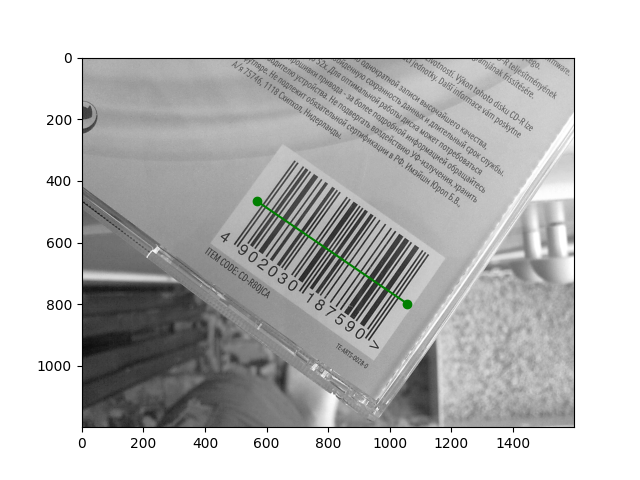
\includegraphics[width=0.5\textwidth]{images/code_barre_couple_vert.png}
	\caption{Segment défini par le deux points en arguments}
	\label{fig:segment}
\end{figure}

Ensuite, la recherche des limites du code-barres amènent à un nouveau segment entre les deux limites. 
Nous obtenons alors le nouveau segment entre les points en rouge sur l'image seuillée, comme illustré sur la figure \ref{fig:binarisation} : 

\begin{figure}[H] 
	\centering
	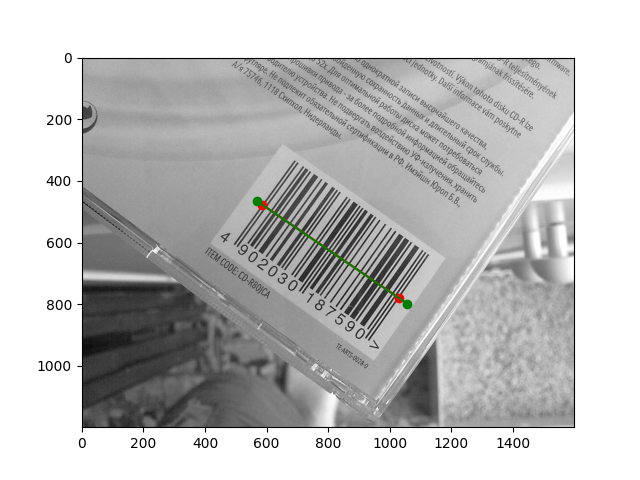
\includegraphics[width=0.5\textwidth]{images/binarisation.png}
	\caption{Nouveau segment produit par l'échantillonnage et la binarisation}
	\label{fig:binarisation}
\end{figure}

Celle-ci montre l'efficacité de la recherche de limites qui correspondent bien à celles observables sur l'image ci-dessus.

\subsubsection*{Analyse du code barre binaire}

On en déduit alors une liste de valeurs binaires. Ceci nous permet ainsi de détecter les zones noires et blanches du code-barres. 
La figure \ref{fig:detection} illustre cette détection, où les zones noires sont représentées en rouge et les zones blanches en bleu.

\begin{figure}[H] 
	\centering
	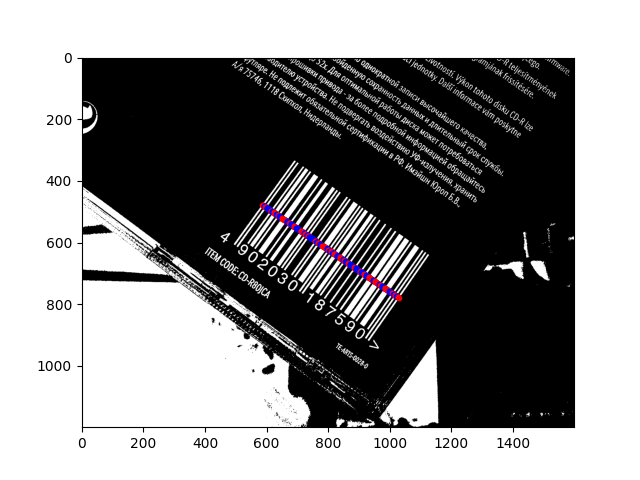
\includegraphics[width=0.5\textwidth]{images/code_seuille_couleur.png}
	\caption{Détection du noir et blanc}
	\label{fig:detection}
\end{figure}

Nous notons ici que le décalage apparent sur l'image n'est que le résultat du dé-zoom de l'image.
À petite échelle, on voit clairement que les zones sont bien détectées (cf Figure \ref{fig:detection_zoom}). 

\begin{figure}[H] 
	\centering
	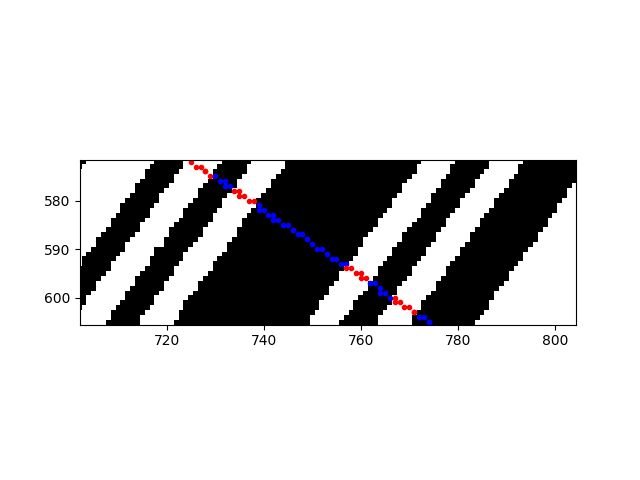
\includegraphics[width=0.5\textwidth]{images/zoom_code_seuille_couleur.png}
	\caption{Zoom de la détection}
	\label{fig:detection_zoom}
\end{figure}

\subsubsection*{Détermination du premier chiffre du code barre}
À l'aide de la séquence AB obtenue, nous pouvons ainsi déterminer le premier chiffre du code barre en se référant au tableau \ref{tab:sequence}.
En l'occurrence, nous obtenons le chiffre \textbf{4} comme premier chiffre. 

\subsubsection*{Vérification de la clef de contrôle}
Nous obtenons alors pour cette image le code \textbf{4902030187590}, ce qui correspond bien au code barre présent sur l'image (cf Figure \ref{code_barre}).
De manière générale, il faut tout de même vérifier la validité du code barre. Pour cela, nous suivons l'algorithme de vérification de code barre grâce à la clé de contrôle.

En l'occurrence, le complément à 10 du dernier chiffre du code barre vaut 0, tandis que le chiffre des unités de la somme des chiffres de rang impair et trois fois la somme des chiffres de rang pair vaut 0. 
Le code barre est donc valide.

\subsection{Unification des algorithmes}

\begin{figure}[H] 
	\begin{center}
    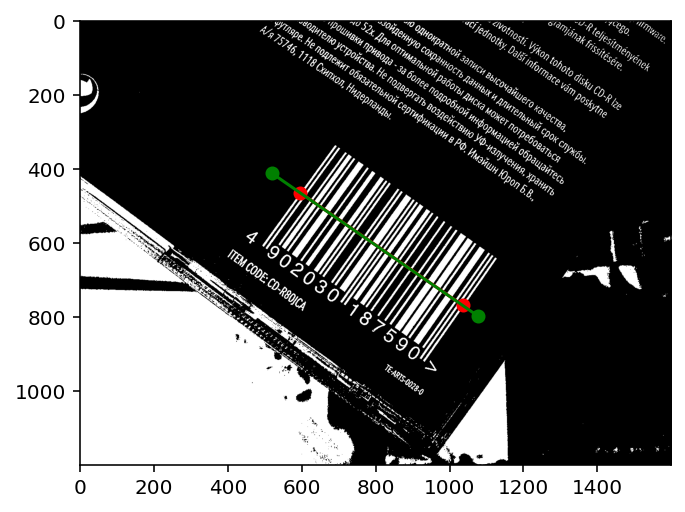
\includegraphics[width=0.7\textwidth]{images/Detection/lecture2.png}
	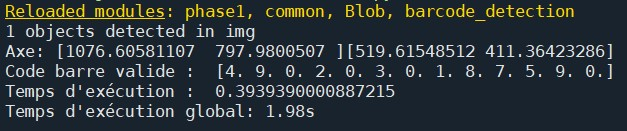
\includegraphics[width=0.7\textwidth]{images/Detection/lecture.jpg}
	\caption{Lecture d'un code barre combinant les deux phases}
	\label{fig:finalres}
    	\end{center}
\end{figure}
En figure \ref{fig:finalres} on observe la sortie obtenue en appliquant l'algorithme de détection qui trace le rayon en vert, utilisé finalement par le programme de lecture.
\newline En combinant ces programmes, on est en mesure, avec des paramètres adéquats à l'image d'effectuer une lecture correcte en un temps de l'ordre de deux secondes.


\newpage 

\section{Conclusion}

\section{Bilan de l'organisation}

\subsection{Séance 1}

\begin{table}[H]
	\centering 
	\begin{tabular}{c|p{12 cm}|c}
		& Tâches entreprises& Temps passé\\ \hline
		Elisa& Prise de connaissance du sujet et commencement de la méthode d'Otsu& 2h\\ \hline
		Alban& Lecture et analyse du sujet et début de l'implémentation d'algorithme d'échantillonnage et de binarisation& 2h\\ \hline
		Tierno & découverte de la problématique, tests sur l'implémentation & 2h\\ \hline
		David & Lecture du sujet et implémentation des différents filtres & 2h \\ \hline
	\end{tabular}
	\caption{Organisation de la séance 1}
\end{table}

\subsection{Séance 2}

\begin{table}[H]
	\centering 
	\begin{tabular}{c|p{12 cm}|c}
		& Tâches entreprises& Temps passé\\ \hline
		Elisa& Finition de la méthode d'Otsu & 2h\\ \hline
		Alban& Complétion de l'échantillonnage et de la binarisation, début du calcul des limites du code-barres et de la recherche de u& 2h\\ \hline
		Tierno & Optimisations et corrections & 3h\\ \hline
		David & Premier prototype de la détection de code barre &  2h \\ \hline
	\end{tabular}
	\caption{Organisation de la séance 2}
\end{table}

\subsection{Séance 3}

\begin{table}[H]
	\centering 
	\begin{tabular}{c|p{12 cm}|c}
		& Tâches entreprises& Temps passé\\ \hline
		Elisa& Débuggage et mise en commun de toutes les fonctions de la phase 1 & 3h\\ \hline
		Alban& Débuggage des fonctions de décodage des blocs fait chez soi et mise en commun du travail phase1& 3h\\ \hline
        % obtention d'un seuillage propre,labelisation
		Tierno & labélisation et extraction des régions d'intérêt & 3h \\ \hline
		David & Implémentation du calcul des couples de points &  3h \\ \hline
	\end{tabular}
	\caption{Organisation de la séance 3}
\end{table}

\subsection{Séance 4}

\begin{table}[H]
	\centering 
	\begin{tabular}{c|p{12 cm}|c}
		& Tâches entreprises& Temps passé\\ \hline
		Elisa& Dernier débuggage et test sur des exemples pour vérifier l'efficacité du code& 3h\\ \hline
		Alban& Dernier débuggage et test sur des exemples pour vérifier l'efficacité du code& 3h\\ \hline
		Tierno & Factorisations, implémentation de la classe Blob (en partie en travail peronnel) & 6h\\ \hline
		David & Mise en commun avec la 2e phase et dernier débuggage &  3h \\ \hline
	\end{tabular}
	\caption{Organisation de la séance 4}
\end{table}

\subsection{Séance 5} % 13 Décembre 

\begin{table}[H]
	\centering 
	\begin{tabular}{c|p{12 cm}|c}
		& Tâches entreprises& Temps passé\\ \hline
		Elisa & Rédaction du rapport & 3h\\ \hline
		Alban & Rédaction du rapport & 3h\\ \hline
		Tierno & Corrections dans l'algorithme de tracé de rayons & 3h\\ \hline
		David& Rédaction du rapport & 3h \\ \hline
	\end{tabular}
	\caption{Organisation de la séance 5}
\end{table}

\newpage

\section{Annexes}

\lstset{style=mystyle}

\subsection{Phase 1 : Détection du code barre}
\subsubsection{Détection des codes barres et tracé de rayons}
\begin{lstlisting}
import numpy as np
import matplotlib.pyplot as plt
from matplotlib import cm
from skimage import io, color, measure
from scipy import signal
from scipy.signal import fftconvolve
from Blob import Blob
from time import time
from math import floor, sqrt
import os
from common import * 
start_time = time()
# ~~~~~~ Fonctions préliminaires ~~~~~~~~~~~~~~~~~~~~~~~~~~~~

def G_2D(sigma):
    x = range(floor(-3*sigma), floor(3*sigma+1))
    X, Y = np.meshgrid(x, x)
    return np.exp(-1/2*(X**2/(sigma**2)+(Y**2/sigma**2)))


def G_x_prime(sigma):  # derive d'une gaussienne
    P = range(floor(-3*sigma), floor(3*sigma+1))
    X, Y = np.meshgrid(P, P)
    return (-X/(2*np.pi*sigma**4)*np.exp(-(X**2+Y**2)/(2*sigma**2)))


def G_y_prime(sigma):  # derive d'une gaussienne
    P = range(floor(-3*sigma), floor(3*sigma+1))
    X, Y = np.meshgrid(P, P)
    return (-Y/(2*np.pi*sigma**4)*np.exp(-(X**2+Y**2)/(2*sigma**2)))

def D(X, Y, Z): return np.sqrt((X-Y)**2+4*Z**2)/(X+Y)

def barcode_detection(img,sigma_g,sigma_t,seuil,sigma_bruit=2,affichage=False):
    # ~~~~~~ Préparation de l'image ~~~~~~~~~~~~~~~~~~~~~~~~~~~~
    # %%
    img_code_barre = plt.imread(img)
    # ~~~~ transformation de rgb en ycrcb  ~~~~~~~~~~~~~~~~~~~
    img_code_barre_YCbCr = color.rgb2ycbcr(img_code_barre)
    Y_code_barre = img_code_barre_YCbCr[:, :, 0]
    Cb_code_barre = img_code_barre_YCbCr[:, :, 1]
    Cr_code_barre = img_code_barre_YCbCr[:, :, 2]
    Y_code_barre += np.random.randn(len(Y_code_barre),len(Y_code_barre[0]))*sigma_bruit
    # ~~~~~~~~~~~~~~~~~~~ Gradients ~~~~~~~~~~~~~~~~~~~
    gauss_x_prime = G_x_prime(sigma_g)
    gauss_y_prime = G_y_prime(sigma_g)
    h, w, c = np.shape(img_code_barre_YCbCr)
    x = np.linspace(0, h, h)
    y = np.linspace(0, w, w)
    X, Y = np.meshgrid(y, x)
    I_x = fftconvolve(Y_code_barre, gauss_x_prime, mode='same')
    I_y = fftconvolve(Y_code_barre, gauss_y_prime, mode='same')
    # ~~~~~ Normalisation ~~~~~~~~~~~~~~~~~~~
    delta_I = np.stack((I_x, I_y), axis=-1)
    N_delta_I = np.linalg.norm(delta_I, ord=2, axis=-1)
    N_I_x = I_x/N_delta_I
    N_I_y = I_y/N_delta_I

    # ~~~~ tenseur de structure local T ~~~~~~~~~~~~~~~~~~~
    gauss2D = G_2D(sigma_t)
    Txx = fftconvolve(N_I_x * N_I_x, gauss2D, mode='same')
    Tyy = fftconvolve(N_I_y * N_I_y, gauss2D, mode='same')
    Txy = fftconvolve(N_I_x * N_I_y, gauss2D, mode='same')
    T = np.block([[Txx, Txy], [Txy, Tyy]])
    # ~~~~ Mesure de cohérence ~~~~~~~~~~~~~~~~~~~~~~~~~~~~
    D_res = D(Txx, Tyy, Txy)
    # ~~~~ Seuillage ~~~~~~~~~~~~~~~~~~~~~~~~~~~~
    D_seuil = (D_res > seuil)
    # ~~~~ Labelisation ~~~~~~~~~~~~~~~~~~~~~~~~~~~~
    D_labeled,num_labels=measure.label(D_seuil,return_num=True)
    blobs=measure.regionprops(D_labeled)
    print(f"{num_labels} objects detected in img")
    coords=[x.coords for x in blobs]
    # ~~~~ Extraction de l'axe ~~~~~~~~~~~~~~~~~~~~~~~~~~~~
    
    # En utilisant la méthode vectorielle
    Blobs=[Blob(pixels=x.coords,imsize=[h,w]) for x in blobs]
    axis=[b.calc_axis_ray(6) for b in Blobs]
    
    # Methode des points extrêmes
    # Blobs=[Blob(pixels=x.coords,imsize=[h,w]) for x in blobs]
    # axis=[b.calc_axis_extr() for b in Blobs]
    #===================================================================
    # affichage basique des rayons obtenus
    plt.figure()
    plt.subplot(1, 2, 1)
    plt.imshow(img_code_barre)
    for blob in Blobs:
        # assert(blob.axis!=None)
        x=[u[0] for u in blob.axis]
        y=[u[1] for u in blob.axis]
        p=blob.barycentre
        plt.plot(p[1],p[0],"or",markersize=2.5)
        plt.plot(x,y,"+b",markersize=5)
    plt.title("img origine")
    plt.subplot(1, 2, 2)
    plt.imshow(D_labeled, cmap=cm.BrBG_r)
    for blob in Blobs:
        # assert(blob.axis!=None)
        x=[u[0] for u in blob.axis]
        y=[u[1] for u in blob.axis]
        p=blob.barycentre
        plt.plot(p[1],p[0],"or",markersize=2.5)
        plt.plot(x,y,"+b",markersize=5)
    plt.title("img labelisee")
    plt.colorbar()
    plt.show()
    if affichage:
        # ~~~~~ Affichage détaillé ~~~~~~~~~~~~~~~~~~~~~~~~~~~~

        plt.figure(1)
        plt.subplot(1, 2, 1)
        plt.imshow(img_code_barre)
        plt.title("img origine")
        plt.subplot(1, 2, 2)
        plt.imshow(img_code_barre_YCbCr[:, :, 0], cmap='gray')
        plt.title("img canal Y")

        plt.figure(2)
        plt.subplot(1, 2, 1)
        plt.imshow(I_x, cmap='gray')
        plt.title("grad x")
        plt.subplot(1, 2, 2)
        plt.imshow(I_y, cmap='gray')
        plt.title("grad y")

        plt.figure(3)
        plt.subplot(1, 2, 1)
        plt.imshow(N_I_x, cmap='gray')
        plt.title("normalisé grad x")
        plt.subplot(1, 2, 2)
        plt.imshow(N_I_y, cmap='gray')
        plt.title("normalisé grad y")

        plt.figure(4)
        plt.subplot(1, 3, 1)
        plt.imshow(Txx, cmap='gray')
        plt.title("Txx")
        plt.subplot(1, 3, 2)
        plt.imshow(Tyy, cmap='gray')
        plt.title("Tyy")
        plt.subplot(1, 3, 3)
        plt.imshow(Txy, cmap='gray')
        plt.title("Txy")

        plt.figure(5)
        plt.subplot(1, 2, 1)
        plt.imshow(D_res, cmap='gray')
        plt.title("D")
        plt.subplot(1, 2, 2)
        plt.imshow(D_seuil, cmap='gray')
        plt.title("D seuil")        
        plt.show()      
    return Blobs
# ~~~~ TEST DE L'EXTRACTION ~~~~~~~~~~~~~~~~~~~~~~~~~~~~
# %%
img="img/barcode0.jpg"
# Pour le bruit, à regler à la main (2 est un bon point de départ)
sigma_bruit = 3

# Pour le gradient, relativement faible pour trouver les vecteurs de transition correspondant aux barres
sigma_g = 2

# Pour le tenseur, relativement élevé pour trouver des clusters de vecteurs gradient
sigma_t = 100

seuil = 0.7 
u=barcode_detection(img,sigma_g,sigma_t,seuil=0.5,sigma_bruit=2)
# u=barcode_detection("img/code_barre_prof.jpg",1,15,0.7,2,affichage=False)
# u=barcode_detection("img/barcode0.jpg",sigma_g=2,sigma_t=50,seuil=0.7,sigma_bruit=2)
# u=barcode_detection("img/b1.jpg",2,50,0.7,2,affichage=False)
for blob in u:
    print("Barycentre: ",end="")
    print(blob.barycentre)
    print("Axe: ",end="")
    print(blob.axis)
    print("Valeurs propres: ",end="")
    print(blob.valeurs_propres)
    o=blob.axis

print(f"Code exécuté en {round(time()-start_time,3)} s")
\end{lstlisting}
\subsubsection{Classe Blob}
\begin{lstlisting}
import numpy as np
import matplotlib.pyplot as plt
from matplotlib import cm
from math import floor, sqrt
from common import *

class Blob:
    def __init__(self, pixels=None,imsize=None):
        # Arguments indispensables
        self.pixels = pixels 
        self.imsize=imsize # (h,w)
        # Calculés ultérieurement
        self.X = None
        self.Y = None
        self.barycentre = None
        self.valeurs_propres = None
        self.vecteurs_propres = None
        self.axis = None
        # Pour d'éventuelles applications futures
        self.area = None
        self.longueur = None
    def calc_XY(self):
        self.X,self.Y=self.pixels[:,0],self.pixels[:,1]
        return self.X,self.Y
    def calc_braycentre(self):
        self.barycentre=np.mean(self.pixels,axis=0)
        return self.barycentre
    def calc_vpropres(self):
        self.valeurs_propres,self.vecteurs_propres=np.linalg.eig(np.cov(self.X,self.Y))
        return self.valeurs_propres,self.vecteurs_propres

    def calc_area(self): # pour éventuellement appliquer un critère de sélection surla taille du bousin
        self.area=self.pixels.size # not the real area, but a good measure of how large it is
        return self.area

    def calc_all(self):
        try:
            self.calc_XY()
            self.calc_braycentre()
            self.calc_vpropres()
            return True
        except Exception as e:
            print(e)
            return False
        
    def calc_axis_0(self):
        self.calc_all()
        if self.axis==None:
            if self.valeurs_propres[0]<self.valeurs_propres[1]:
                p1 = floor(self.barycentre[1]+self.valeurs_propres[0]/2*self.vecteurs_propres[0][0]), floor(self.barycentre[0]+self.valeurs_propres[0]/2*self.vecteurs_propres[0][1])
                p2 = floor(self.barycentre[1]-self.valeurs_propres[0]/2*self.vecteurs_propres[0][0]), floor(self.barycentre[0]-self.valeurs_propres[0]/2*self.vecteurs_propres[0][1])
                self.axis=[p1,p2]
            else:
                p1 = floor(self.barycentre[1]+self.valeurs_propres[1]/2*self.vecteurs_propres[1][0]), floor(self.barycentre[0]+self.valeurs_propres[1]/2*self.vecteurs_propres[1][1])
                p2 = floor(self.barycentre[1]-self.valeurs_propres[1]/2*self.vecteurs_propres[1][0]), floor(self.barycentre[0]-self.valeurs_propres[1]/2*self.vecteurs_propres[1][1])
                self.axis=[p1,p2]
        return self.axis
    
    def calc_axis_extr(self):
        # méthode des points extrêmes
        self.calc_all()
        if self.axis==None:
            max_l=max(self.imsize)
            if self.valeurs_propres[0]<self.valeurs_propres[1]:
                vecteurs_propres_norm=self.vecteurs_propres[0]/np.linalg.norm(self.vecteurs_propres[0])
                p1 = floor(self.barycentre[1]+max_l*vecteurs_propres_norm[0]), floor(self.barycentre[0]+max_l*vecteurs_propres_norm[1])
                p2 = floor(self.barycentre[1]-max_l*vecteurs_propres_norm[0]), floor(self.barycentre[0]-max_l*vecteurs_propres_norm[1])
                p1=bornage(self.imsize[1],self.imsize[0],p1)
                p2=bornage(self.imsize[1],self.imsize[0],p2)
                self.axis=[p1,p2]
            else:
                vecteurs_propres_norm=self.vecteurs_propres[1]/np.linalg.norm(self.vecteurs_propres[1])
                p1 = floor(self.barycentre[1]+max_l*vecteurs_propres_norm[0]), floor(self.barycentre[0]+max_l*vecteurs_propres_norm[1])
                p2 = floor(self.barycentre[1]-max_l*vecteurs_propres_norm[0]), floor(self.barycentre[0]-max_l*vecteurs_propres_norm[1])
                p1=bornage(self.imsize[1],self.imsize[0],p1)
                p2=bornage(self.imsize[1],self.imsize[0],p2)
                self.axis=[p1,p2]
        return self.axis
    
    def calc_axis_ray(self,len_adjust=6):
        # len adjust: facteur d'ajustement pour la longueur finale de l'axe. initialement à 1.
        self.calc_all()
        if self.valeurs_propres[0]>self.valeurs_propres[1]: #on détecte la valeur propre la plus grande
            imax=0 
        else:
            imax=1
        axe=np.abs(self.vecteurs_propres[:,(imax+1)%2]) #on extrait le vecteur propre correspondant à la valeur minimale
        # abs pour etre sur d'extraire le bon angle
        axe_norm=axe/np.linalg.norm(axe,2) 
        alpha=np.arccos(axe_norm[0]) # on extrait l'angle avec l'horizontale
        r=len_adjust*np.sqrt(self.valeurs_propres[imax])
        self.axis = ray_center(self.barycentre[::-1],r , alpha) 
        return self.axis
        
    def draw_random_rays(self,length,n):
        self.calc_all()
        return [random_ray_center_2(self.imsize[0], self.imsize[1], length, self.barycentre) for i in range(n)]
    
\end{lstlisting}
\subsubsection{Fonctions utilitaires}
\begin{lstlisting}
import numpy as np
import matplotlib.pyplot as plt

def bornage(h, w, p): # à voir si une accélération est possible
    p=list(p)
    if p[0] < 0:
        p[0] = 0
    if p[0] > h:
        p[0] = h-1
    if p[1] < 0:
        p[1] = 0
    if p[1] > w:
        p[1] = w-1
    return p

# ~~~~ Fonctions tracé de rayons ~~~~~~~~~~~~~~~~~~~~~~~~~~~~
# %%
# ajouter des paramètres pour avoir un tirage gaussien (ou autre)

def ray_center(center,length,angle):
    """
    Parameters
    ----------
    center : np.array([x0,y0])
    length : float
    angle : float
    crée un rayon de centre center, de longueur length et d'angle alpha (par rapport à l'horizontale)
    """
    offset = np.array([np.cos(angle), np.sin(angle)])*length/2
    x1 = center+offset
    x2 = center-offset
    return np.array([x1,x2])

def random_ray_center(h, w, length):
    # méthode: centre, angle, longueur
    angle = np.random.uniform(0, 2*np.pi)
    r = length/2
    center = np.array([np.random.randint(0, h), np.random.randint(0, w)])
    offset = np.array([np.cos(angle), np.sin(angle)])*r
    x1 = center+offset
    x2 = center-offset
    return np.int32([bornage(h, w, x1), bornage(h, w, x2)])
    
def random_ray_center_2(h, w, length,center):
    # méthode: centre, angle, longueur
    angle = np.random.uniform(0, 2*np.pi)
    r = length/2
    offset = np.array([np.cos(angle), np.sin(angle)])*r
    x1 = center+offset
    x2 = center-offset
    return np.int32([bornage(h, w, x1), bornage(h, w, x2)])
    
def random_ray(h, w, length):
    # méthode: extrémité1, angle, longueur
    angle = np.random.uniform(0, 2*np.pi)

    x1 = np.array([np.random.randint(0, h), np.random.randint(0, w)])
    offset = np.array([np.cos(angle), np.sin(angle)])*length
    x2 = x1+offset

    return np.int32([bornage(h, w, x1), bornage(h, w, x2)])

def plot_ray(ray):
    # for debugging
    plt.figure()
    plt.plot(ray[:,0],ray[:,1])
    k=5
    plt.plot(k * np.array([1, 1, -1, -1, 1]), k * np.array([1, -1, -1, 1, 1]))
    plt.grid()
    return
 
def get_angle(ray):
    ray=np.array(ray)
    print(ray)
    axe=np.abs(ray[:,1]-ray[:,0]) #abs pour être sûr d'extraire l'angle avec l'horizontale
    axe_norm=axe/np.linalg.norm(axe,2) 
    alpha=np.arccos(axe_norm[0]) # on extrait l'angle avec l'horizontale
    return alpha
\end{lstlisting}
\subsection{Phase 2 : Lecture du code barre}
\begin{lstlisting}
def otsu(img, bins=255):
	luminance = None
	
	# Si l'image est en couleur (3 dimensions)
	if len(img.shape) == 3 and img.shape[2] > 1:
		# Calcul de la luminance 
		luminance = np.array([[(img[i][j][0] + img[i][j][1] + img[i][j][2])//3 for j in range(img.shape[1])] for i in range(img.shape[0])])
		luminance = luminance.ravel()
	else:
		luminance = img.ravel()
	
	# Création de l'histogramme
	histogram, bin_edges = np.histogram(luminance.ravel(), range=(0, 255), bins=bins)
	
	# Moyenner l'histogramme
	histogram = histogram/sum(histogram)    
	
	# Création d'un dico pour associer chaque valeur de luminance à sa fréquence
	histogram_dic = {int(bin_edges[i]): histogram[i] for i in range(len(histogram))}
	
	# Initialisation des moyennes et poids initiaux
	n = len(histogram_dic)
	sumB = 0
	wB = 0
	maximum = 0.0
	sum1 = sum(i * histogram_dic[i] for i in range(n))
	total = sum(histogram_dic.values())
	level = 0
	for k in range(1, n):
		wF = total - wB
		if wB > 0 and wF > 0:
			mF = (sum1 - sumB) / wF
			val = wB * wF * (sumB / wB - mF) * (sumB / wB - mF)
			
			if val >= maximum:
				level = k
				maximum = val
		
		wB += histogram_dic[k]
		sumB += (k-1) * histogram_dic[k] # A vérifier si c'est k ou k-1
	
	return level

def distance(x1,y1,x2,y2):
	""" Calcule la distance entre deux points """
	return np.sqrt((x2-x1)**2+(y2-y1)**2)

def echantillonnage(x1,y1,x2,y2,Nb_points):
	"""On échantillone sur le segment (x1,y1)->(x2,y2)"""
	"""On va choisir le plus proche voisin"""
	X=np.around(np.linspace(np.floor(x1),np.ceil(x2),Nb_points)).astype(int)
	Y=np.around(np.linspace(np.floor(y1),np.ceil(y2),Nb_points)).astype(int)
	return X,Y


def find_lim(x1,y1,x2,y2,img,seuil):
    """Récupération des points de départ et d'arrivée pour le segment 2"""
    X,Y=echantillonnage(x1,y1,x2,y2,np.ceil(distance(x1, y1, x2, y2)).astype(int))
    valeurs_img=np.zeros((len(X), 1))

    for i in range(0,len(X)):
        valeurs_img[i]=(img[Y[i], X[i]]) >= seuil
    i1=0
    i2=0

    for i in range(0,len(valeurs_img)):
        if valeurs_img[i]==0:
            i1=i
            break
    for i in range(len(valeurs_img)-1,1,-1):
        if valeurs_img[i]==0:
            i2=i
            break
    return X[i1],Y[i1],X[i2],Y[i2] # xd,yd,xa,ya


def find_u(xd,yd,xa,ya,img,seuil):
    """On va prendre le multiple u et le signal binaire à analyser"""
    nb_p=np.ceil(distance(xd,yd,xa,ya)).astype(int) # Nombre de points L'
    Nb_points=0 # u * 95
    u=0
    while (Nb_points<=nb_p): # On cherche le plus petit u tq u * 95 > nb_p
        Nb_points+=95
        u+=1
    
    X,Y=echantillonnage(xd,yd,xa,ya,Nb_points)
    valeurs_img=np.zeros((len(X), 1))
    
    for i in range(0,len(X)):
        valeurs_img[i]=(img[Y[i], X[i]]) <= seuil
    

    return valeurs_img,u #Echantillonnage et binarisation


def separate(segment_seuille,u):
    L=np.zeros((12,u*7))
    start=3*u # Détermine les "gardes" (offset)
    for i in range(0,12):
        if (i==6):
            start=start+5*u
        segment_seuille_temp = segment_seuille[start+i*7*u : start+(i+1)*7*u]

        for j in range(len(L[i])):
            L[i,j] = segment_seuille_temp[j,0]  

    return L

def norme_binaire(liste_binaire,chaine_binaire,u):
    sum=0
    for k in range(0,7):
        for i in range(0,u):
            sum+=(liste_binaire[k*u+i]!=int(chaine_binaire[k]))
    return sum

def compare(region_chiffres_bin,L_the,u):
    normes_codes=len(region_chiffres_bin[0])
    decode=np.zeros((12))
    r=""
    for i in range(0,6):
        r_b=r
        for j in range(0,len(L_the[0])):
            if (normes_codes>=norme_binaire(region_chiffres_bin[i],L_the[0][j],u)):
                normes_codes=norme_binaire(region_chiffres_bin[i],L_the[0][j],u)
                decode[i]=int(j)
                r=r_b+"A"
            if (normes_codes>=norme_binaire(region_chiffres_bin[i],L_the[1][j],u)):
                normes_codes=norme_binaire(region_chiffres_bin[i],L_the[1][j],u)
                decode[i]=int(j)
                r=r_b+"B"
        normes_codes=len(region_chiffres_bin[0])
    for i in range(6,len(region_chiffres_bin)):
        for j in range(0,len(L_the[0])):
            if (normes_codes>=norme_binaire(region_chiffres_bin[i],L_the[2][j],u)):
                normes_codes=norme_binaire(region_chiffres_bin[i],L_the[2][j],u)
                decode[i]=int(j)
        normes_codes=len(region_chiffres_bin[0])
    return decode,r


def first_one(decode,r,tab):
    """ Retourne le premier chiffre """
    for i in range(0,len(tab)):
        if (r==tab[i]):
            return i
    return None

def clef_controle(decode):
    # Complément à 10 du dernier chiffre du code barre
    complement = (10 - decode[-1]) % 10

    L = [1, 3, 1, 3, 1, 3, 1, 3, 1, 3, 1, 3]
    clef = np.sum(decode[0:-1] * L) % 10
    return clef == complement

def phase1(x, y, img, seuil):
    starttime = time.perf_counter()
    x1 = x[0]
    y1 = y[0]
    x2 = x[1]
    y2 = y[1]
    codage_chiffres_bin = [["0001101", "0011001", "0010011", "0111101", "0100011", "0110001", "0101111", "0111011", "0110111", "0001011"],
                           ["0100111", "0110011", "0011011", "0100001", "0011101", "0111001", "0000101", "0010001", "0001001", "0010111"],
                           ["1110010", "1100110", "1101100", "1000010", "1011100", "1001110", "1010000", "1000100", "1001000", "1110100"]]
    codage_premier_chiffre = ["AAAAAA","AABABB","AABBAB","AABBBA","ABAABB","ABBAAB","ABBBAA","ABABAB","ABABBA","ABBABA"]
    Nb=np.ceil(distance(x1, y1, x2, y2)).astype(int) # Nombre de points
    
    # Binarisation
    xd,yd,xa,ya = find_lim(x1,y1,x2,y2,img,seuil)
    
    # Echantillonage + Binarisation de l'image après seuillage 
    segment_seuillage, u = find_u(xd,yd,xa,ya,img,seuil)
    regions_chiffres_bin = separate(segment_seuillage,u)
    
    # Décodage des regions binaires
    regions_chiffres, sequence_AB = compare(regions_chiffres_bin,codage_chiffres_bin,u)
    
    # Ajout du premier chiffre
    premier_chiffre = first_one(regions_chiffres,sequence_AB,codage_premier_chiffre)
    
    if (premier_chiffre == None):
        return None
    
    code_barre = np.append(premier_chiffre, regions_chiffres)
    
    # Vérification de la clé de contrôle
    if clef_controle(code_barre):
        print("Code barre valide : ", code_barre)
        endtime = time.perf_counter() - starttime
        print("Temps d'exécution : ", endtime)
        return code_barre
    else:
        print("Code barre invalide : ", code_barre)
        return None 

\end{lstlisting}
\subsection{Main}
\begin{lstlisting}
from phase1 import *
from barcode_detection import *
start=time()
# Détection des barres
img_name = 'img/barcode0.jpg'

# Lecture du code barre 
img = cv2.imread(img_name, cv2.IMREAD_GRAYSCALE)

# Seuillage avec la méthode d'Otsu
seuil = otsu(img)

# Extraction des points d'intérêt
Blobs = barcode_detection(img_name, sigma_g=2, sigma_t=50, seuil=0.7, sigma_bruit=2)
# Lecture à partir des points trouvés
for blob in Blobs:
    # altérer la méthode de calcul de l'axe si besoin (blob.calc_axis_...)
    # blob.calc_axis_ray(len_adjust=5)
    x = blob.axis[:,0].astype(int).tolist()[::-1]
    y = blob.axis[:,1].astype(int).tolist()[::-1]
    print("Axe: ", end="")
    print(blob.axis[0], end=""); print(blob.axis[1])
    res=phase1(x, y, img, seuil)

duration=time()-start
print("Temps d'exécution global: {}s".format(round(duration,2)))
\end{lstlisting}
\end{document}